% !TEX root = ../../prj4projektrapport.tex
% SKAL STÅ I TOPPEN AF ALLE FILER FOR AT MASTER-filen KOMPILERES 

For at Spændingsregulatoren kan foretage en regulering af spændingen i systemet, skal den løbende have informationer om de reelle forhold i nettet. Denne information står Måleenheden for at indsamle. Måleenhedens opgave er at måle spænding, strøm, indhold af harmoniske og power faktor. I kapitlet vil der blive redegjort for hvilke løsninger er valgt for at opnå den ønskede funktionalitet. 

\section{Foranalyse}
Det var først tænkt at købe nogle sensorer til PLC'en der kunne måle de ønskede værdier. Men da PLC'en ikke kan sample hurtigt nok til at give et reelt billede af signalet, er der valgt at bruge en PSOC til at sample signalet. Derefter kan værdierne sendes til Styringsenheden. Måleenheden er tænkt til at skulle måle differentielt som vist på figur \ref{fig:MaalForanalyse}. Spændingen måles over forbrugeren og 1$\Omega$ modstand, hvor strømmen måles som spændingen over den 1$\Omega$ modstand.

\begin{figure}[H] % (alternativt [H])
	\centering
	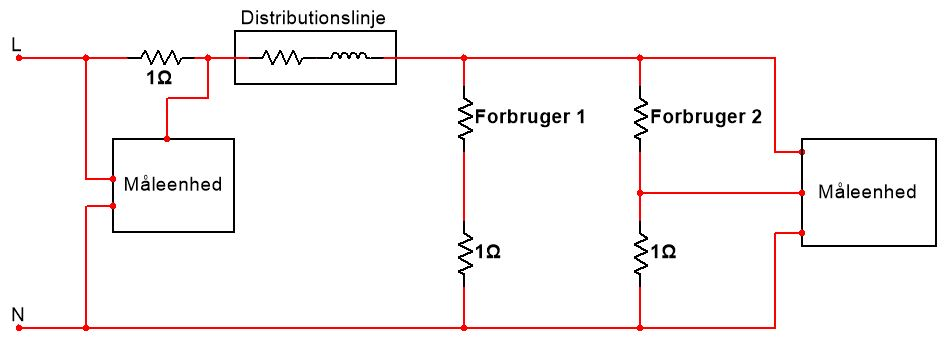
\includegraphics[width=0.8\textwidth]{figure/MaalForanalyse}
	\caption{Tænkt tilslutning af måleenhed}
	\label{fig:MaalForanalyse}
\end{figure}

\section{Signal behandling}

Iht. Shannons samplings teori\cite{Shannon}, kan der ses et reelt billede af et signal, når samplings frekvensen er dobbelt så stor som selve signalet. Da systemet er proof of concept, er det besluttet kun at aflæse på de fire første harmoniske til 50Hz signalet. Det vil sige at der undersøges, hvor meget energi der er i frekvenserne 100, 150, 200 og 250Hz. Det betyder at der minimum skal samples med 500Hz i projektet.

Når et signalet er samplet til det digitale spektrum, kan signalet analyseres. Til at undersøge signalernes størrelse, power faktor og indhold af harmoniske kan Fourier anvendes. Ved at lave Fourier på en række samplede værdier, fås en ny række komplekse tal. Hvert kompleks tal, angiver værdien for en bestemt frekvens i et signal, der kaldes for frekvens bins. Ud fra denne komplekse værdi kan størrelsen og fasevinklen ved bestemte frekvenser findes. Det anvendes i projektet til at beregne rms værdier af spænding og strøm for 50Hz, men også vinklen mellem spænding og strøm der giver udtryk for power faktoren. Derudover kan signalet også undersøges i højere frekvenser så indhold af harmoniske kan udregnes.  

